\begin{enunciado}{\ejExtra}
  Sean $S_1 = \ket{(2,1,3)}$ y $S_2 = \ket{(4,2,6), (1,0,4)}$.
  \begin{enumerate}[label=\alph*)]
    \item Mostrar que $S_1 \subset S_2$.

    \item Sea $P$ el proyector ortogonal sobre $S_2$. Probar que $S_1 \subset \nucleo(I - P^T)$.

    \item Calcular la distancia de (-2, 6, 4) a $S_2$ usando P(-2, 6, 4).
  \end{enumerate}
\end{enunciado}

\begin{enumerate}[label=\alph*)]
  \item Busco ecuación  de $S_2$:
        $$
          a (4,2,6) + b (1,0,4) = (x_1, x_2, x_3)
          \flecha{armo sistema}
          \matriz{cc|c}{
            4 & 1 & x_1 \\
            2 & 0 & x_2 \\
            6 & 4 & x_3
          }
        $$
        resolviendo ese sistema obtengo:
        $$
          B_S = \set{(x_1, x_2, x_3) \en \reales^3 / -8x_1 + 10x_2 + 2x_3 = 0}
        $$
        Saco de paso y barato mirando los coeficientes de la ecuación de $S$:
        $$
          B_{S^\perp} = \set{(-4, 5, 1)}
        $$

        Volviendo al ejercicio ¿$S_1 \subset S_2$?: Sí, porque cumple la ecuación del subespacio.

  \item La papa está acá $I - P_{S_2}^t$, un \textit{proyector ortogonal} cumple que su expresión matricial es simétrica:
        $$
          I - P_{S_2}^t = I - P_{S_2}
        $$
        Por lo tanto si quiero buscar ver si un vector pertenece al núcleo de $I- \nucleo(P_{S_2})$:
        $$
          S_1 \subset S_2
          \entonces
          P_{S_2}(S_1) = S_1
        $$
        Por lo tanto:
        $$
          (I - P_{S_2})S_1 = S_1 - P_{S_2}S_1 = S_1 - S_1 = 0
        $$

  \item
        La distancia la puedo calcular como :
        $$
          \norma{(-2,6,4) - P_{S_2}(-2,6,4)}
        $$
        Calculo una BON para $S_2$ y $S_2^\perp$:
        $$
          BON_{S_2} =
          \set{
            \left(-\frac{1}{\sqrt{3}}, -\frac{1}{\sqrt{3}}, \frac{1}{\sqrt{3}}\right),
            \left(\frac{2}{\sqrt{14}}, \frac{1}{\sqrt{14}}, \frac{3}{\sqrt{14}}\right)
          }
        $$
        $$
          BON_{S_2^\perp} =
          \set{
            \left(-\frac{4}{\sqrt{42}}, \frac{1}{\sqrt{42}}, \frac{2}{\sqrt{42}}\right)
          }
        $$
        $$
          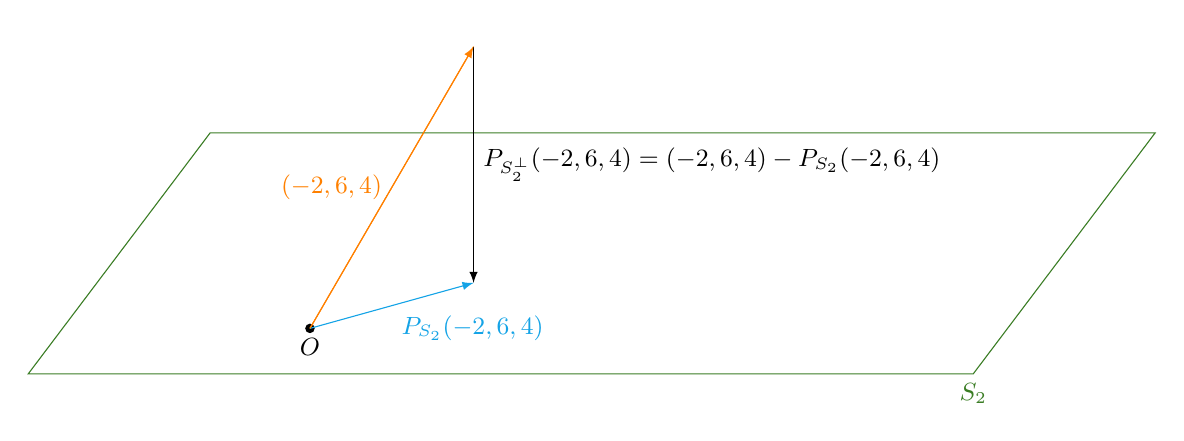
\begin{tikzpicture}[scale = 1.5, every node/.style={font=\small}]
            \coordinate[] (A) at (-1,0.5,0);
            \coordinate[] (B) at (-1,0,4);
            \coordinate[] (C) at (7,0,4);
            \coordinate[] (D) at (7,0.5,0);
            \coordinate[] (P) at (2,2,2);
            \coordinate[] (O) at (1,0,3);
            \coordinate[] (PP) at (2,0,2);
            \filldraw[] (O) circle[radius = 1pt] node[below]{$O$};
            \draw[orange] (O) -- (P) node[midway, left]{$(-2,6,4)$};
            \draw[OliveGreen] (A)--(B)--(C)node[below]{$S_2$}--(D)--cycle;
            \draw[thin,-latex, black] (P)--(PP) node[midway,right]{$P_{S_2^\perp}(-2,6,4) = (-2,6,4) - P_{S_2}(-2,6,4)$} ;
            \draw[thin,-latex, Cerulean] (O)--(PP) node[midway, below right]{$P_{S_2}(-2,6,4)$} ;
            \draw[-latex,orange] (O)--(P) node[above left]{};
          \end{tikzpicture}
        $$
        Viendo el gráfico conviene calcular para hacer quinientas cuentas menos:
        $$
          \textstyle
          \norma{P_{S_2^\perp}\orange{(-2,6,4)}} =
          \norma{
            \Big(
            \ub{
              \orange{(-2, 6, 4)}
              \cdot
              \big(-\frac{4}{\sqrt{42}}, \frac{1}{\sqrt{42}}, \frac{2}{\sqrt{42}}\big)
            }{\frac{22}{\sqrt{42}}}
            \Big)
            \Big(
            \big(-\frac{4}{\sqrt{42}}, \frac{1}{\sqrt{42}}, \frac{2}{\sqrt{42}}\big)
            \Big)
          }
          =
          \norma{(\frac{44}{21}, \frac{11}{21}, \frac{22}{21})}
        $$
        Por lo tanto la distancia buscada:
        $$
          d((-2,6,4), S_2) = \frac{11}{\sqrt{21}}
        $$
        Oka, decía usando $\blue{P_{S_2}}$, pero, pero...{\color{black!10!white}{ me chupa un huevo.}}

        Pero bueh, ahí queda la base $BON_{S_2} = \set{v_1, v_2}$, calculá con \orange{$v = (-2, 4, 6)$}:
        $$
          P_{S_2}(\orange{v}) = (v_1 \cdot \orange{v}) \cdot v_1 + (v_2 \cdot \orange{v}) \cdot v_2
        $$
        eso sería la proyección azul del gráfico, entonces para calcular la longitud del vector negro:
        $$
          \norma{\orange{v} -  \blue{(v_1 \cdot v) \cdot v_1 + (v_2 \cdot v) \cdot v_2 }} = d(\orange{(-2,6,4), \green{S_2}})
        $$
\end{enumerate}

\begin{aportes}
  \item \aporte{\dirRepo}{naD GarRaz \github}
\end{aportes}
